\documentclass[1p]{elsarticle_modified}
%\bibliographystyle{elsarticle-num}

%\usepackage[colorlinks]{hyperref}
%\usepackage{abbrmath_seonhwa} %\Abb, \Ascr, \Acal ,\Abf, \Afrak
\usepackage{amsfonts}
\usepackage{amssymb}
\usepackage{amsmath}
\usepackage{amsthm}
\usepackage{scalefnt}
\usepackage{amsbsy}
\usepackage{kotex}
\usepackage{caption}
\usepackage{subfig}
\usepackage{color}
\usepackage{graphicx}
\usepackage{xcolor} %% white, black, red, green, blue, cyan, magenta, yellow
\usepackage{float}
\usepackage{setspace}
\usepackage{hyperref}

\usepackage{tikz}
\usetikzlibrary{arrows}

\usepackage{multirow}
\usepackage{array} % fixed length table
\usepackage{hhline}

%%%%%%%%%%%%%%%%%%%%%
\makeatletter
\renewcommand*\env@matrix[1][\arraystretch]{%
	\edef\arraystretch{#1}%
	\hskip -\arraycolsep
	\let\@ifnextchar\new@ifnextchar
	\array{*\c@MaxMatrixCols c}}
\makeatother %https://tex.stackexchange.com/questions/14071/how-can-i-increase-the-line-spacing-in-a-matrix
%%%%%%%%%%%%%%%

\usepackage[normalem]{ulem}

\newcommand{\msout}[1]{\ifmmode\text{\sout{\ensuremath{#1}}}\else\sout{#1}\fi}
%SOURCE: \msout is \stkout macro in https://tex.stackexchange.com/questions/20609/strikeout-in-math-mode

\newcommand{\cancel}[1]{
	\ifmmode
	{\color{red}\msout{#1}}
	\else
	{\color{red}\sout{#1}}
	\fi
}

\newcommand{\add}[1]{
	{\color{blue}\uwave{#1}}
}

\newcommand{\replace}[2]{
	\ifmmode
	{\color{red}\msout{#1}}{\color{blue}\uwave{#2}}
	\else
	{\color{red}\sout{#1}}{\color{blue}\uwave{#2}}
	\fi
}

\newcommand{\Sol}{\mathcal{S}} %segment
\newcommand{\D}{D} %diagram
\newcommand{\A}{\mathcal{A}} %arc


%%%%%%%%%%%%%%%%%%%%%%%%%%%%%5 test

\def\sl{\operatorname{\textup{SL}}(2,\Cbb)}
\def\psl{\operatorname{\textup{PSL}}(2,\Cbb)}
\def\quan{\mkern 1mu \triangleright \mkern 1mu}

\theoremstyle{definition}
\newtheorem{thm}{Theorem}[section]
\newtheorem{prop}[thm]{Proposition}
\newtheorem{lem}[thm]{Lemma}
\newtheorem{ques}[thm]{Question}
\newtheorem{cor}[thm]{Corollary}
\newtheorem{defn}[thm]{Definition}
\newtheorem{exam}[thm]{Example}
\newtheorem{rmk}[thm]{Remark}
\newtheorem{alg}[thm]{Algorithm}

\newcommand{\I}{\sqrt{-1}}
\begin{document}

%\begin{frontmatter}
%
%\title{Boundary parabolic representations of knots up to 8 crossings}
%
%%% Group authors per affiliation:
%\author{Yunhi Cho} 
%\address{Department of Mathematics, University of Seoul, Seoul, Korea}
%\ead{yhcho@uos.ac.kr}
%
%
%\author{Seonhwa Kim} %\fnref{s_kim}}
%\address{Center for Geometry and Physics, Institute for Basic Science, Pohang, 37673, Korea}
%\ead{ryeona17@ibs.re.kr}
%
%\author{Hyuk Kim}
%\address{Department of Mathematical Sciences, Seoul National University, Seoul 08826, Korea}
%\ead{hyukkim@snu.ac.kr}
%
%\author{Seokbeom Yoon}
%\address{Department of Mathematical Sciences, Seoul National University, Seoul, 08826,  Korea}
%\ead{sbyoon15@snu.ac.kr}
%
%\begin{abstract}
%We find all boundary parabolic representation of knots up to 8 crossings.
%
%\end{abstract}
%\begin{keyword}
%    \MSC[2010] 57M25 
%\end{keyword}
%
%\end{frontmatter}

%\linenumbers
%\tableofcontents
%
\newcommand\colored[1]{\textcolor{white}{\rule[-0.35ex]{0.8em}{1.4ex}}\kern-0.8em\color{red} #1}%
%\newcommand\colored[1]{\textcolor{white}{ #1}\kern-2.17ex	\textcolor{white}{ #1}\kern-1.81ex	\textcolor{white}{ #1}\kern-2.15ex\color{red}#1	}

{\Large $\underline{12n_{0262}~(K12n_{0262})}$}

\setlength{\tabcolsep}{10pt}
\renewcommand{\arraystretch}{1.6}
\vspace{1cm}\begin{tabular}{m{100pt}>{\centering\arraybackslash}m{274pt}}
\multirow{5}{120pt}{
	\centering
	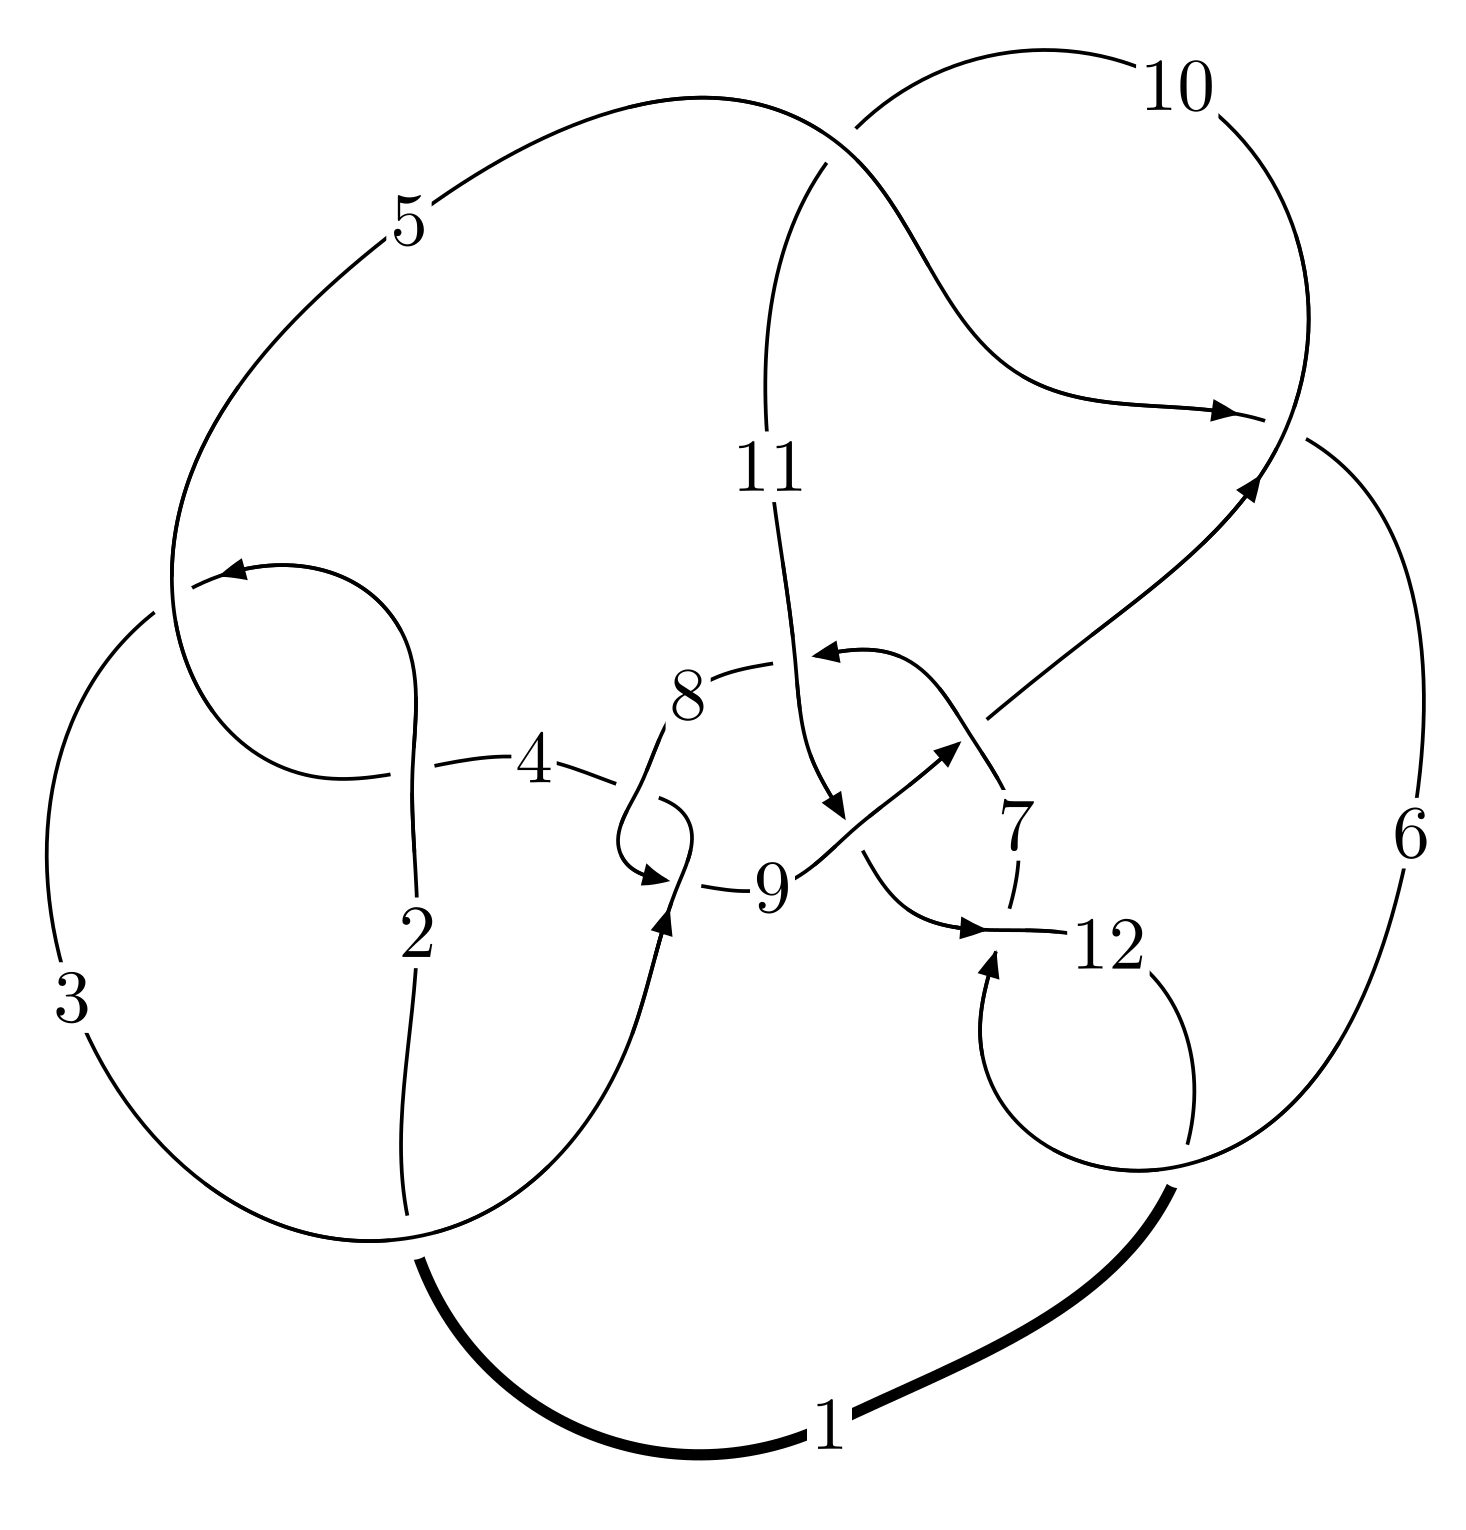
\includegraphics[width=112pt]{../../../GIT/diagram.site/Diagrams/png/2351_12n_0262.png}\\
\ \ \ A knot diagram\footnotemark}&
\allowdisplaybreaks
\textbf{Linearized knot diagam} \\
\cline{2-2}
 &
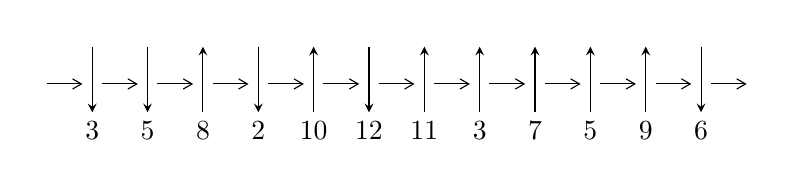
\begin{tikzpicture}[x=20pt, y=17pt]
	% nodes
	\node (C0) at (0, 0) {};
	\node (C1) at (1, 0) {};
	\node (C1U) at (1, +1) {};
	\node (C1D) at (1, -1) {3};

	\node (C2) at (2, 0) {};
	\node (C2U) at (2, +1) {};
	\node (C2D) at (2, -1) {5};

	\node (C3) at (3, 0) {};
	\node (C3U) at (3, +1) {};
	\node (C3D) at (3, -1) {8};

	\node (C4) at (4, 0) {};
	\node (C4U) at (4, +1) {};
	\node (C4D) at (4, -1) {2};

	\node (C5) at (5, 0) {};
	\node (C5U) at (5, +1) {};
	\node (C5D) at (5, -1) {10};

	\node (C6) at (6, 0) {};
	\node (C6U) at (6, +1) {};
	\node (C6D) at (6, -1) {12};

	\node (C7) at (7, 0) {};
	\node (C7U) at (7, +1) {};
	\node (C7D) at (7, -1) {11};

	\node (C8) at (8, 0) {};
	\node (C8U) at (8, +1) {};
	\node (C8D) at (8, -1) {3};

	\node (C9) at (9, 0) {};
	\node (C9U) at (9, +1) {};
	\node (C9D) at (9, -1) {7};

	\node (C10) at (10, 0) {};
	\node (C10U) at (10, +1) {};
	\node (C10D) at (10, -1) {5};

	\node (C11) at (11, 0) {};
	\node (C11U) at (11, +1) {};
	\node (C11D) at (11, -1) {9};

	\node (C12) at (12, 0) {};
	\node (C12U) at (12, +1) {};
	\node (C12D) at (12, -1) {6};
	\node (C13) at (13, 0) {};

	% arrows
	\draw[->,>={angle 60}]
	(C0) edge (C1) (C1) edge (C2) (C2) edge (C3) (C3) edge (C4) (C4) edge (C5) (C5) edge (C6) (C6) edge (C7) (C7) edge (C8) (C8) edge (C9) (C9) edge (C10) (C10) edge (C11) (C11) edge (C12) (C12) edge (C13) ;	\draw[->,>=stealth]
	(C1U) edge (C1D) (C2U) edge (C2D) (C3D) edge (C3U) (C4U) edge (C4D) (C5D) edge (C5U) (C6U) edge (C6D) (C7D) edge (C7U) (C8D) edge (C8U) (C9D) edge (C9U) (C10D) edge (C10U) (C11D) edge (C11U) (C12U) edge (C12D) ;
	\end{tikzpicture} \\
\hhline{~~} \\& 
\textbf{Solving Sequence} \\ \cline{2-2} 
 &
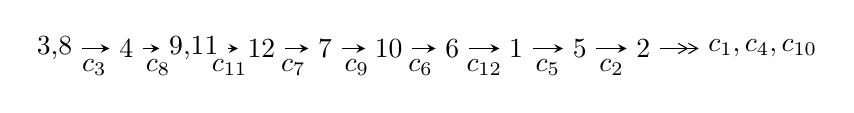
\begin{tikzpicture}[x=23pt, y=7pt]
	% node
	\node (A0) at (-1/8, 0) {3,8};
	\node (A1) at (1, 0) {4};
	\node (A2) at (33/16, 0) {9,11};
	\node (A3) at (25/8, 0) {12};
	\node (A4) at (33/8, 0) {7};
	\node (A5) at (41/8, 0) {10};
	\node (A6) at (49/8, 0) {6};
	\node (A7) at (57/8, 0) {1};
	\node (A8) at (65/8, 0) {5};
	\node (A9) at (73/8, 0) {2};
	\node (C1) at (1/2, -1) {$c_{3}$};
	\node (C2) at (3/2, -1) {$c_{8}$};
	\node (C3) at (21/8, -1) {$c_{11}$};
	\node (C4) at (29/8, -1) {$c_{7}$};
	\node (C5) at (37/8, -1) {$c_{9}$};
	\node (C6) at (45/8, -1) {$c_{6}$};
	\node (C7) at (53/8, -1) {$c_{12}$};
	\node (C8) at (61/8, -1) {$c_{5}$};
	\node (C9) at (69/8, -1) {$c_{2}$};
	\node (A10) at (11, 0) {$c_{1},c_{4},c_{10}$};

	% edge
	\draw[->,>=stealth]	
	(A0) edge (A1) (A1) edge (A2) (A2) edge (A3) (A3) edge (A4) (A4) edge (A5) (A5) edge (A6) (A6) edge (A7) (A7) edge (A8) (A8) edge (A9) ;
	\draw[->>,>={angle 60}]	
	(A9) edge (A10);
\end{tikzpicture} \\ 

\end{tabular} \\

\footnotetext{
The image of knot diagram is generated by the software ``\textbf{Draw programme}" developed by Andrew Bartholomew(\url{http://www.layer8.co.uk/maths/draw/index.htm\#Running-draw}), where we modified some parts for our purpose(\url{https://github.com/CATsTAILs/LinksPainter}).
}\phantom \\ \newline 
\centering \textbf{Ideals for irreducible components\footnotemark of $X_{\text{par}}$} 
 
\begin{align*}
I^u_{1}&=\langle 
-1.84691\times10^{298} u^{66}-1.95567\times10^{298} u^{65}+\cdots+2.05840\times10^{302} b+1.32241\times10^{302},\\
\phantom{I^u_{1}}&\phantom{= \langle  }1.98179\times10^{298} u^{66}+3.24951\times10^{298} u^{65}+\cdots+4.11679\times10^{302} a-1.22918\times10^{303},\\
\phantom{I^u_{1}}&\phantom{= \langle  }u^{67}+u^{66}+\cdots+43008 u-25088\rangle \\
I^u_{2}&=\langle 
-5673781 u^{13}-878483 u^{12}+\cdots+3057583 b+1514771,\\
\phantom{I^u_{2}}&\phantom{= \langle  }-2814143 u^{13}-1845304 u^{12}+\cdots+3057583 a-4471166,\\
\phantom{I^u_{2}}&\phantom{= \langle  }u^{14}+3 u^{12}-3 u^{11}-5 u^{10}+4 u^9-11 u^8+8 u^7+12 u^6+8 u^5+20 u^4+6 u^2- u+1\rangle \\
\\
I^v_{1}&=\langle 
a,\;-579074 v^8+1101995 v^7+\cdots+5353327 b+7952402,\\
\phantom{I^v_{1}}&\phantom{= \langle  }v^9- v^8-8 v^7+v^6+33 v^5+23 v^4-14 v^3-2 v^2+3 v-7\rangle \\
\end{align*}
\raggedright * 3 irreducible components of $\dim_{\mathbb{C}}=0$, with total 90 representations.\\
\footnotetext{All coefficients of polynomials are rational numbers. But the coefficients are sometimes approximated in decimal forms when there is not enough margin.}
\newpage
\renewcommand{\arraystretch}{1}
\centering \section*{I. $I^u_{1}= \langle -1.85\times10^{298} u^{66}-1.96\times10^{298} u^{65}+\cdots+2.06\times10^{302} b+1.32\times10^{302},\;1.98\times10^{298} u^{66}+3.25\times10^{298} u^{65}+\cdots+4.12\times10^{302} a-1.23\times10^{303},\;u^{67}+u^{66}+\cdots+43008 u-25088 \rangle$}
\flushleft \textbf{(i) Arc colorings}\\
\begin{tabular}{m{7pt} m{180pt} m{7pt} m{180pt} }
\flushright $a_{3}=$&$\begin{pmatrix}1\\0\end{pmatrix}$ \\
\flushright $a_{8}=$&$\begin{pmatrix}0\\u\end{pmatrix}$ \\
\flushright $a_{4}=$&$\begin{pmatrix}1\\- u^2\end{pmatrix}$ \\
\flushright $a_{9}=$&$\begin{pmatrix}u\\u\end{pmatrix}$ \\
\flushright $a_{11}=$&$\begin{pmatrix}-0.0000481392 u^{66}-0.0000789331 u^{65}+\cdots+5.33036 u+2.98578\\0.0000897259 u^{66}+0.0000950094 u^{65}+\cdots-2.62585 u-0.642448\end{pmatrix}$ \\
\flushright $a_{12}=$&$\begin{pmatrix}-0.000118460 u^{66}-0.000172623 u^{65}+\cdots+7.23750 u+3.89089\\0.0000194055 u^{66}+1.31979\times10^{-6} u^{65}+\cdots-0.718714 u+0.262662\end{pmatrix}$ \\
\flushright $a_{7}=$&$\begin{pmatrix}0.000161293 u^{66}+0.000149952 u^{65}+\cdots-9.45357 u+1.04345\\0.0000806828 u^{66}+0.000116961 u^{65}+\cdots+1.08719 u-2.12829\end{pmatrix}$ \\
\flushright $a_{10}=$&$\begin{pmatrix}-0.000137853 u^{66}-0.000195770 u^{65}+\cdots+3.84559 u+4.00787\\0.0000222838 u^{66}+0.0000208994 u^{65}+\cdots+1.86058 u-0.321979\end{pmatrix}$ \\
\flushright $a_{6}=$&$\begin{pmatrix}0.000161217 u^{66}+0.000186979 u^{65}+\cdots-5.83761 u-2.26918\\0.000148461 u^{66}+0.000256361 u^{65}+\cdots+2.53370 u-6.92210\end{pmatrix}$ \\
\flushright $a_{1}=$&$\begin{pmatrix}-0.0000197759 u^{66}-0.0000240684 u^{65}+\cdots+1.14983 u+0.135437\\-3.32757\times10^{-6} u^{66}+1.67327\times10^{-7} u^{65}+\cdots+0.785198 u-0.156001\end{pmatrix}$ \\
\flushright $a_{5}=$&$\begin{pmatrix}0.0000164483 u^{66}+0.0000242357 u^{65}+\cdots-0.364631 u-0.291438\\-7.60200\times10^{-6} u^{66}-7.07139\times10^{-6} u^{65}+\cdots+0.707461 u-0.351370\end{pmatrix}$ \\
\flushright $a_{2}=$&$\begin{pmatrix}-0.0000164483 u^{66}-0.0000242357 u^{65}+\cdots+0.364631 u+0.291438\\-3.32757\times10^{-6} u^{66}+1.67327\times10^{-7} u^{65}+\cdots+0.785198 u-0.156001\end{pmatrix}$\\&\end{tabular}
\flushleft \textbf{(ii) Obstruction class $= -1$}\\~\\
\flushleft \textbf{(iii) Cusp Shapes $= 0.000336583 u^{66}+0.000559671 u^{65}+\cdots-0.882700 u-3.59196$}\\~\\
\newpage\renewcommand{\arraystretch}{1}
\flushleft \textbf{(iv) u-Polynomials at the component}\newline \\
\begin{tabular}{m{50pt}|m{274pt}}
Crossings & \hspace{64pt}u-Polynomials at each crossing \\
\hline $$\begin{aligned}c_{1}\end{aligned}$$&$\begin{aligned}
&u^{67}+78 u^{66}+\cdots+171200 u+2401
\end{aligned}$\\
\hline $$\begin{aligned}c_{2},c_{4}\end{aligned}$$&$\begin{aligned}
&u^{67}-16 u^{66}+\cdots+120 u-49
\end{aligned}$\\
\hline $$\begin{aligned}c_{3},c_{8}\end{aligned}$$&$\begin{aligned}
&u^{67}+u^{66}+\cdots+43008 u-25088
\end{aligned}$\\
\hline $$\begin{aligned}c_{5},c_{10}\end{aligned}$$&$\begin{aligned}
&u^{67}-2 u^{66}+\cdots+3200 u-773
\end{aligned}$\\
\hline $$\begin{aligned}c_{6},c_{12}\end{aligned}$$&$\begin{aligned}
&u^{67}-3 u^{66}+\cdots+781 u-209
\end{aligned}$\\
\hline $$\begin{aligned}c_{7}\end{aligned}$$&$\begin{aligned}
&u^{67}+u^{66}+\cdots+566773 u-256243
\end{aligned}$\\
\hline $$\begin{aligned}c_{9}\end{aligned}$$&$\begin{aligned}
&u^{67}+4 u^{66}+\cdots-2 u-1
\end{aligned}$\\
\hline $$\begin{aligned}c_{11}\end{aligned}$$&$\begin{aligned}
&u^{67}+12 u^{66}+\cdots-77902 u-10969
\end{aligned}$\\
\hline
\end{tabular}\\~\\
\newpage\renewcommand{\arraystretch}{1}
\flushleft \textbf{(v) Riley Polynomials at the component}\newline \\
\begin{tabular}{m{50pt}|m{274pt}}
Crossings & \hspace{64pt}Riley Polynomials at each crossing \\
\hline $$\begin{aligned}c_{1}\end{aligned}$$&$\begin{aligned}
&y^{67}-162 y^{66}+\cdots+5062883876 y-5764801
\end{aligned}$\\
\hline $$\begin{aligned}c_{2},c_{4}\end{aligned}$$&$\begin{aligned}
&y^{67}-78 y^{66}+\cdots+171200 y-2401
\end{aligned}$\\
\hline $$\begin{aligned}c_{3},c_{8}\end{aligned}$$&$\begin{aligned}
&y^{67}+63 y^{66}+\cdots-2491940864 y-629407744
\end{aligned}$\\
\hline $$\begin{aligned}c_{5},c_{10}\end{aligned}$$&$\begin{aligned}
&y^{67}+62 y^{66}+\cdots-18480042 y-597529
\end{aligned}$\\
\hline $$\begin{aligned}c_{6},c_{12}\end{aligned}$$&$\begin{aligned}
&y^{67}+33 y^{66}+\cdots-240251 y-43681
\end{aligned}$\\
\hline $$\begin{aligned}c_{7}\end{aligned}$$&$\begin{aligned}
&y^{67}+43 y^{66}+\cdots+161121782381 y-65660475049
\end{aligned}$\\
\hline $$\begin{aligned}c_{9}\end{aligned}$$&$\begin{aligned}
&y^{67}-10 y^{66}+\cdots-44 y-1
\end{aligned}$\\
\hline $$\begin{aligned}c_{11}\end{aligned}$$&$\begin{aligned}
&y^{67}+16 y^{66}+\cdots-1081596550 y-120318961
\end{aligned}$\\
\hline
\end{tabular}\\~\\
\newpage\flushleft \textbf{(vi) Complex Volumes and Cusp Shapes}
$$\begin{array}{c|c|c}  
\text{Solutions to }I^u_{1}& \I (\text{vol} + \sqrt{-1}CS) & \text{Cusp shape}\\
 \hline 
\begin{aligned}
u &= -0.972237 + 0.280854 I \\
a &= -0.933702 - 0.142151 I \\
b &= -0.109882 - 0.192634 I\end{aligned}
 & \phantom{-}3.39425 - 2.09087 I & \phantom{-}8.43522 + 3.94985 I \\ \hline\begin{aligned}
u &= -0.972237 - 0.280854 I \\
a &= -0.933702 + 0.142151 I \\
b &= -0.109882 + 0.192634 I\end{aligned}
 & \phantom{-}3.39425 + 2.09087 I & \phantom{-}8.43522 - 3.94985 I \\ \hline\begin{aligned}
u &= -0.111044 + 1.030770 I \\
a &= \phantom{-}0.537195 + 0.271868 I \\
b &= \phantom{-}1.82570 + 1.10431 I\end{aligned}
 & \phantom{-}0.89656 - 5.19617 I & \phantom{-}2.00000 + 8.56770 I \\ \hline\begin{aligned}
u &= -0.111044 - 1.030770 I \\
a &= \phantom{-}0.537195 - 0.271868 I \\
b &= \phantom{-}1.82570 - 1.10431 I\end{aligned}
 & \phantom{-}0.89656 + 5.19617 I & \phantom{-}2.00000 - 8.56770 I \\ \hline\begin{aligned}
u &= \phantom{-}0.502448 + 0.771343 I \\
a &= \phantom{-}0.284361 + 0.812390 I \\
b &= \phantom{-}0.879173 + 0.333242 I\end{aligned}
 & \phantom{-}0.42745 + 2.04731 I & \phantom{-}1.79133 - 2.30943 I \\ \hline\begin{aligned}
u &= \phantom{-}0.502448 - 0.771343 I \\
a &= \phantom{-}0.284361 - 0.812390 I \\
b &= \phantom{-}0.879173 - 0.333242 I\end{aligned}
 & \phantom{-}0.42745 - 2.04731 I & \phantom{-}1.79133 + 2.30943 I \\ \hline\begin{aligned}
u &= -0.163401 + 0.813880 I \\
a &= -0.463100 + 0.420844 I \\
b &= -1.144220 + 0.605865 I\end{aligned}
 & -1.58473 + 1.12240 I & -2.95098 - 3.87144 I \\ \hline\begin{aligned}
u &= -0.163401 - 0.813880 I \\
a &= -0.463100 - 0.420844 I \\
b &= -1.144220 - 0.605865 I\end{aligned}
 & -1.58473 - 1.12240 I & -2.95098 + 3.87144 I \\ \hline\begin{aligned}
u &= -0.687972 + 0.429990 I \\
a &= -0.466340 + 0.203651 I \\
b &= -0.705353 - 0.489291 I\end{aligned}
 & -2.34582 + 0.79184 I & -1.70277 + 1.36728 I \\ \hline\begin{aligned}
u &= -0.687972 - 0.429990 I \\
a &= -0.466340 - 0.203651 I \\
b &= -0.705353 + 0.489291 I\end{aligned}
 & -2.34582 - 0.79184 I & -1.70277 - 1.36728 I\\
 \hline 
 \end{array}$$\newpage$$\begin{array}{c|c|c}  
\text{Solutions to }I^u_{1}& \I (\text{vol} + \sqrt{-1}CS) & \text{Cusp shape}\\
 \hline 
\begin{aligned}
u &= -0.423056 + 1.121960 I \\
a &= -0.340034 + 1.265540 I \\
b &= -0.758978 + 0.645501 I\end{aligned}
 & -4.49098 - 4.90499 I & \phantom{-0.000000 } 0 \\ \hline\begin{aligned}
u &= -0.423056 - 1.121960 I \\
a &= -0.340034 - 1.265540 I \\
b &= -0.758978 - 0.645501 I\end{aligned}
 & -4.49098 + 4.90499 I & \phantom{-0.000000 } 0 \\ \hline\begin{aligned}
u &= -0.683441 + 0.994440 I \\
a &= -0.700678 + 0.584635 I \\
b &= -1.65806 - 0.19823 I\end{aligned}
 & -2.72054 + 1.47592 I & \phantom{-0.000000 } 0 \\ \hline\begin{aligned}
u &= -0.683441 - 0.994440 I \\
a &= -0.700678 - 0.584635 I \\
b &= -1.65806 + 0.19823 I\end{aligned}
 & -2.72054 - 1.47592 I & \phantom{-0.000000 } 0 \\ \hline\begin{aligned}
u &= \phantom{-}0.412259 + 0.668041 I \\
a &= -0.952707 + 0.932487 I \\
b &= -2.33800 + 1.37488 I\end{aligned}
 & \phantom{-}0.01538 + 1.90218 I & \phantom{-}1.03416 - 1.99152 I \\ \hline\begin{aligned}
u &= \phantom{-}0.412259 - 0.668041 I \\
a &= -0.952707 - 0.932487 I \\
b &= -2.33800 - 1.37488 I\end{aligned}
 & \phantom{-}0.01538 - 1.90218 I & \phantom{-}1.03416 + 1.99152 I \\ \hline\begin{aligned}
u &= -0.734728 + 0.191087 I \\
a &= -1.088980 - 0.815803 I \\
b &= -0.029495 + 0.284816 I\end{aligned}
 & \phantom{-}3.56178 + 1.95197 I & \phantom{-}9.44446 - 1.83557 I \\ \hline\begin{aligned}
u &= -0.734728 - 0.191087 I \\
a &= -1.088980 + 0.815803 I \\
b &= -0.029495 - 0.284816 I\end{aligned}
 & \phantom{-}3.56178 - 1.95197 I & \phantom{-}9.44446 + 1.83557 I \\ \hline\begin{aligned}
u &= \phantom{-}0.705362 + 0.112303 I \\
a &= \phantom{-}0.447657 - 0.096628 I \\
b &= -0.57181 - 1.47755 I\end{aligned}
 & -0.78374 + 3.24647 I & \phantom{-}3.36554 - 8.05825 I \\ \hline\begin{aligned}
u &= \phantom{-}0.705362 - 0.112303 I \\
a &= \phantom{-}0.447657 + 0.096628 I \\
b &= -0.57181 + 1.47755 I\end{aligned}
 & -0.78374 - 3.24647 I & \phantom{-}3.36554 + 8.05825 I\\
 \hline 
 \end{array}$$\newpage$$\begin{array}{c|c|c}  
\text{Solutions to }I^u_{1}& \I (\text{vol} + \sqrt{-1}CS) & \text{Cusp shape}\\
 \hline 
\begin{aligned}
u &= \phantom{-}0.489130 + 0.496557 I \\
a &= \phantom{-}0.999235 + 0.996408 I \\
b &= \phantom{-}1.080650 + 0.076642 I\end{aligned}
 & \phantom{-}0.85096 + 2.02536 I & \phantom{-}5.69785 - 3.31418 I \\ \hline\begin{aligned}
u &= \phantom{-}0.489130 - 0.496557 I \\
a &= \phantom{-}0.999235 - 0.996408 I \\
b &= \phantom{-}1.080650 - 0.076642 I\end{aligned}
 & \phantom{-}0.85096 - 2.02536 I & \phantom{-}5.69785 + 3.31418 I \\ \hline\begin{aligned}
u &= \phantom{-}0.058657 + 0.664653 I \\
a &= \phantom{-}0.66387 - 2.11195 I \\
b &= \phantom{-}1.24815 - 0.75030 I\end{aligned}
 & \phantom{-}0.17719 - 3.22158 I & -2.38086 + 5.47011 I \\ \hline\begin{aligned}
u &= \phantom{-}0.058657 - 0.664653 I \\
a &= \phantom{-}0.66387 + 2.11195 I \\
b &= \phantom{-}1.24815 + 0.75030 I\end{aligned}
 & \phantom{-}0.17719 + 3.22158 I & -2.38086 - 5.47011 I \\ \hline\begin{aligned}
u &= \phantom{-}0.028062 + 0.629541 I \\
a &= \phantom{-}1.38866 + 0.32024 I \\
b &= \phantom{-}1.85271 - 1.86384 I\end{aligned}
 & -3.79798 - 0.21805 I & -3.18632 - 4.76372 I \\ \hline\begin{aligned}
u &= \phantom{-}0.028062 - 0.629541 I \\
a &= \phantom{-}1.38866 - 0.32024 I \\
b &= \phantom{-}1.85271 + 1.86384 I\end{aligned}
 & -3.79798 + 0.21805 I & -3.18632 + 4.76372 I \\ \hline\begin{aligned}
u &= \phantom{-}0.580709 + 0.074213 I \\
a &= -1.64498 + 1.24717 I \\
b &= \phantom{-}0.1199620 + 0.0262995 I\end{aligned}
 & \phantom{-}2.35238 - 6.89299 I & \phantom{-}11.67033 + 2.73841 I \\ \hline\begin{aligned}
u &= \phantom{-}0.580709 - 0.074213 I \\
a &= -1.64498 - 1.24717 I \\
b &= \phantom{-}0.1199620 - 0.0262995 I\end{aligned}
 & \phantom{-}2.35238 + 6.89299 I & \phantom{-}11.67033 - 2.73841 I \\ \hline\begin{aligned}
u &= -0.568924 + 0.015800 I \\
a &= \phantom{-}1.15399 - 1.27396 I \\
b &= -0.137363 - 0.361208 I\end{aligned}
 & -2.33563 - 2.09946 I & \phantom{-}2.27732 + 3.69468 I \\ \hline\begin{aligned}
u &= -0.568924 - 0.015800 I \\
a &= \phantom{-}1.15399 + 1.27396 I \\
b &= -0.137363 + 0.361208 I\end{aligned}
 & -2.33563 + 2.09946 I & \phantom{-}2.27732 - 3.69468 I\\
 \hline 
 \end{array}$$\newpage$$\begin{array}{c|c|c}  
\text{Solutions to }I^u_{1}& \I (\text{vol} + \sqrt{-1}CS) & \text{Cusp shape}\\
 \hline 
\begin{aligned}
u &= -0.22902 + 1.42563 I \\
a &= -1.41393 + 0.24587 I \\
b &= -1.77271 + 0.17285 I\end{aligned}
 & -4.88346 - 3.38279 I & \phantom{-0.000000 } 0 \\ \hline\begin{aligned}
u &= -0.22902 - 1.42563 I \\
a &= -1.41393 - 0.24587 I \\
b &= -1.77271 - 0.17285 I\end{aligned}
 & -4.88346 + 3.38279 I & \phantom{-0.000000 } 0 \\ \hline\begin{aligned}
u &= -0.06118 + 1.47148 I \\
a &= -1.178520 - 0.232850 I \\
b &= -1.81942 - 0.53750 I\end{aligned}
 & -7.03108 - 4.31642 I & \phantom{-0.000000 } 0 \\ \hline\begin{aligned}
u &= -0.06118 - 1.47148 I \\
a &= -1.178520 + 0.232850 I \\
b &= -1.81942 + 0.53750 I\end{aligned}
 & -7.03108 + 4.31642 I & \phantom{-0.000000 } 0 \\ \hline\begin{aligned}
u &= -0.116938 + 0.471533 I \\
a &= \phantom{-}1.76704 + 0.77132 I \\
b &= \phantom{-}0.88022 + 1.53954 I\end{aligned}
 & \phantom{-}0.98108 + 2.41958 I & \phantom{-}3.63595 + 0.97039 I \\ \hline\begin{aligned}
u &= -0.116938 - 0.471533 I \\
a &= \phantom{-}1.76704 - 0.77132 I \\
b &= \phantom{-}0.88022 - 1.53954 I\end{aligned}
 & \phantom{-}0.98108 - 2.41958 I & \phantom{-}3.63595 - 0.97039 I \\ \hline\begin{aligned}
u &= \phantom{-}1.50349 + 0.34050 I \\
a &= \phantom{-}0.256622 - 0.478404 I \\
b &= \phantom{-}0.222034 + 0.138144 I\end{aligned}
 & \phantom{-}2.74618 + 3.31023 I & \phantom{-0.000000 } 0 \\ \hline\begin{aligned}
u &= \phantom{-}1.50349 - 0.34050 I \\
a &= \phantom{-}0.256622 + 0.478404 I \\
b &= \phantom{-}0.222034 - 0.138144 I\end{aligned}
 & \phantom{-}2.74618 - 3.31023 I & \phantom{-0.000000 } 0 \\ \hline\begin{aligned}
u &= \phantom{-}1.55291 + 0.23943 I \\
a &= -0.163132 - 1.062710 I \\
b &= \phantom{-}0.084878 - 0.518349 I\end{aligned}
 & -8.96576 + 1.05371 I & \phantom{-0.000000 } 0 \\ \hline\begin{aligned}
u &= \phantom{-}1.55291 - 0.23943 I \\
a &= -0.163132 + 1.062710 I \\
b &= \phantom{-}0.084878 + 0.518349 I\end{aligned}
 & -8.96576 - 1.05371 I & \phantom{-0.000000 } 0\\
 \hline 
 \end{array}$$\newpage$$\begin{array}{c|c|c}  
\text{Solutions to }I^u_{1}& \I (\text{vol} + \sqrt{-1}CS) & \text{Cusp shape}\\
 \hline 
\begin{aligned}
u &= -0.52715 + 1.48204 I \\
a &= \phantom{-}0.916886 - 0.098363 I \\
b &= \phantom{-}1.357000 - 0.270061 I\end{aligned}
 & -6.16260 - 2.01828 I & \phantom{-0.000000 } 0 \\ \hline\begin{aligned}
u &= -0.52715 - 1.48204 I \\
a &= \phantom{-}0.916886 + 0.098363 I \\
b &= \phantom{-}1.357000 + 0.270061 I\end{aligned}
 & -6.16260 + 2.01828 I & \phantom{-0.000000 } 0 \\ \hline\begin{aligned}
u &= \phantom{-}0.413083\phantom{ +0.000000I} \\
a &= \phantom{-}1.65958\phantom{ +0.000000I} \\
b &= \phantom{-}0.141582\phantom{ +0.000000I}\end{aligned}
 & \phantom{-}0.931638\phantom{ +0.000000I} & \phantom{-}11.2120\phantom{ +0.000000I} \\ \hline\begin{aligned}
u &= \phantom{-}0.14745 + 1.66191 I \\
a &= -0.15458 - 1.63422 I \\
b &= -0.348487 - 0.802841 I\end{aligned}
 & -8.02419 + 4.33010 I & \phantom{-0.000000 } 0 \\ \hline\begin{aligned}
u &= \phantom{-}0.14745 - 1.66191 I \\
a &= -0.15458 + 1.63422 I \\
b &= -0.348487 + 0.802841 I\end{aligned}
 & -8.02419 - 4.33010 I & \phantom{-0.000000 } 0 \\ \hline\begin{aligned}
u &= \phantom{-}0.45724 + 1.63971 I \\
a &= -0.794772 - 0.109984 I \\
b &= -1.92407 + 0.56192 I\end{aligned}
 & -6.70242 + 8.43737 I & \phantom{-0.000000 } 0 \\ \hline\begin{aligned}
u &= \phantom{-}0.45724 - 1.63971 I \\
a &= -0.794772 + 0.109984 I \\
b &= -1.92407 - 0.56192 I\end{aligned}
 & -6.70242 - 8.43737 I & \phantom{-0.000000 } 0 \\ \hline\begin{aligned}
u &= \phantom{-}0.05684 + 1.70857 I \\
a &= -0.671485 + 0.613787 I \\
b &= -1.194770 - 0.506092 I\end{aligned}
 & -12.22050 + 0.78224 I & \phantom{-0.000000 } 0 \\ \hline\begin{aligned}
u &= \phantom{-}0.05684 - 1.70857 I \\
a &= -0.671485 - 0.613787 I \\
b &= -1.194770 + 0.506092 I\end{aligned}
 & -12.22050 - 0.78224 I & \phantom{-0.000000 } 0 \\ \hline\begin{aligned}
u &= -0.13255 + 1.73913 I \\
a &= \phantom{-}0.910845 + 0.114746 I \\
b &= \phantom{-}1.80242 + 0.30695 I\end{aligned}
 & -10.39740 - 2.64649 I & \phantom{-0.000000 } 0\\
 \hline 
 \end{array}$$\newpage$$\begin{array}{c|c|c}  
\text{Solutions to }I^u_{1}& \I (\text{vol} + \sqrt{-1}CS) & \text{Cusp shape}\\
 \hline 
\begin{aligned}
u &= -0.13255 - 1.73913 I \\
a &= \phantom{-}0.910845 - 0.114746 I \\
b &= \phantom{-}1.80242 - 0.30695 I\end{aligned}
 & -10.39740 + 2.64649 I & \phantom{-0.000000 } 0 \\ \hline\begin{aligned}
u &= \phantom{-}0.41326 + 1.75472 I \\
a &= \phantom{-}0.961322 - 0.083022 I \\
b &= \phantom{-}1.83983 - 0.48405 I\end{aligned}
 & -5.00803 + 10.48120 I & \phantom{-0.000000 } 0 \\ \hline\begin{aligned}
u &= \phantom{-}0.41326 - 1.75472 I \\
a &= \phantom{-}0.961322 + 0.083022 I \\
b &= \phantom{-}1.83983 + 0.48405 I\end{aligned}
 & -5.00803 - 10.48120 I & \phantom{-0.000000 } 0 \\ \hline\begin{aligned}
u &= \phantom{-}0.65145 + 1.69788 I \\
a &= \phantom{-}1.342150 - 0.141007 I \\
b &= \phantom{-}2.08846 - 0.33679 I\end{aligned}
 & -14.9522 + 8.9665 I & \phantom{-0.000000 } 0 \\ \hline\begin{aligned}
u &= \phantom{-}0.65145 - 1.69788 I \\
a &= \phantom{-}1.342150 + 0.141007 I \\
b &= \phantom{-}2.08846 + 0.33679 I\end{aligned}
 & -14.9522 - 8.9665 I & \phantom{-0.000000 } 0 \\ \hline\begin{aligned}
u &= \phantom{-}0.92464 + 1.58340 I \\
a &= -0.930597 + 0.161778 I \\
b &= -1.45672 + 0.17040 I\end{aligned}
 & -12.8012 + 7.6595 I & \phantom{-0.000000 } 0 \\ \hline\begin{aligned}
u &= \phantom{-}0.92464 - 1.58340 I \\
a &= -0.930597 - 0.161778 I \\
b &= -1.45672 - 0.17040 I\end{aligned}
 & -12.8012 - 7.6595 I & \phantom{-0.000000 } 0 \\ \hline\begin{aligned}
u &= -0.91168 + 1.66821 I \\
a &= -1.132070 - 0.045052 I \\
b &= -2.09892 - 0.39558 I\end{aligned}
 & -12.2648 - 16.4135 I & \phantom{-0.000000 } 0 \\ \hline\begin{aligned}
u &= -0.91168 - 1.66821 I \\
a &= -1.132070 + 0.045052 I \\
b &= -2.09892 + 0.39558 I\end{aligned}
 & -12.2648 + 16.4135 I & \phantom{-0.000000 } 0 \\ \hline\begin{aligned}
u &= \phantom{-}0.07685 + 1.90361 I \\
a &= -0.784906 + 0.030539 I \\
b &= -1.58347 - 0.28609 I\end{aligned}
 & -5.56017 - 2.92233 I & \phantom{-0.000000 } 0\\
 \hline 
 \end{array}$$\newpage$$\begin{array}{c|c|c}  
\text{Solutions to }I^u_{1}& \I (\text{vol} + \sqrt{-1}CS) & \text{Cusp shape}\\
 \hline 
\begin{aligned}
u &= \phantom{-}0.07685 - 1.90361 I \\
a &= -0.784906 - 0.030539 I \\
b &= -1.58347 + 0.28609 I\end{aligned}
 & -5.56017 + 2.92233 I & \phantom{-0.000000 } 0 \\ \hline\begin{aligned}
u &= -1.91592 + 0.19283 I \\
a &= \phantom{-}0.014025 + 0.880781 I \\
b &= -0.347688 + 0.042615 I\end{aligned}
 & -7.74590 + 6.82406 I & \phantom{-0.000000 } 0 \\ \hline\begin{aligned}
u &= -1.91592 - 0.19283 I \\
a &= \phantom{-}0.014025 - 0.880781 I \\
b &= -0.347688 - 0.042615 I\end{aligned}
 & -7.74590 - 6.82406 I & \phantom{-0.000000 } 0 \\ \hline\begin{aligned}
u &= -0.29235 + 2.06576 I \\
a &= \phantom{-}0.585168 + 0.348851 I \\
b &= \phantom{-}1.75404 - 0.52002 I\end{aligned}
 & -13.6589 - 4.4760 I & \phantom{-0.000000 } 0 \\ \hline\begin{aligned}
u &= -0.29235 - 2.06576 I \\
a &= \phantom{-}0.585168 - 0.348851 I \\
b &= \phantom{-}1.75404 + 0.52002 I\end{aligned}
 & -13.6589 + 4.4760 I & \phantom{-0.000000 } 0 \\ \hline\begin{aligned}
u &= -0.73570 + 2.03169 I \\
a &= \phantom{-}0.755689 + 0.211036 I \\
b &= \phantom{-}1.67913 + 0.00462 I\end{aligned}
 & -14.4098 - 3.1017 I & \phantom{-0.000000 } 0 \\ \hline\begin{aligned}
u &= -0.73570 - 2.03169 I \\
a &= \phantom{-}0.755689 - 0.211036 I \\
b &= \phantom{-}1.67913 - 0.00462 I\end{aligned}
 & -14.4098 + 3.1017 I & \phantom{-0.000000 } 0\\
 \hline 
 \end{array}$$\newpage\newpage\renewcommand{\arraystretch}{1}
\centering \section*{II. $I^u_{2}= \langle -5.67\times10^{6} u^{13}-8.78\times10^{5} u^{12}+\cdots+3.06\times10^{6} b+1.51\times10^{6},\;-2.81\times10^{6} u^{13}-1.85\times10^{6} u^{12}+\cdots+3.06\times10^{6} a-4.47\times10^{6},\;u^{14}+3 u^{12}+\cdots- u+1 \rangle$}
\flushleft \textbf{(i) Arc colorings}\\
\begin{tabular}{m{7pt} m{180pt} m{7pt} m{180pt} }
\flushright $a_{3}=$&$\begin{pmatrix}1\\0\end{pmatrix}$ \\
\flushright $a_{8}=$&$\begin{pmatrix}0\\u\end{pmatrix}$ \\
\flushright $a_{4}=$&$\begin{pmatrix}1\\- u^2\end{pmatrix}$ \\
\flushright $a_{9}=$&$\begin{pmatrix}u\\u\end{pmatrix}$ \\
\flushright $a_{11}=$&$\begin{pmatrix}0.920382 u^{13}+0.603517 u^{12}+\cdots+2.27554 u+1.46232\\1.85564 u^{13}+0.287313 u^{12}+\cdots+6.16967 u-0.495415\end{pmatrix}$ \\
\flushright $a_{12}=$&$\begin{pmatrix}0.936012 u^{13}+0.704950 u^{12}+\cdots+1.02408 u+1.77852\\1.87127 u^{13}+0.388745 u^{12}+\cdots+4.91821 u-0.179210\end{pmatrix}$ \\
\flushright $a_{7}=$&$\begin{pmatrix}-0.154016 u^{13}+0.0867479 u^{12}+\cdots+5.44332 u-0.520875\\0.238361 u^{13}+0.739303 u^{12}+\cdots+6.37952 u-0.597333\end{pmatrix}$ \\
\flushright $a_{10}=$&$\begin{pmatrix}0.920382 u^{13}+0.603517 u^{12}+\cdots+3.27554 u+1.46232\\1.88950 u^{13}+0.545803 u^{12}+\cdots+6.90949 u+0.157140\end{pmatrix}$ \\
\flushright $a_{6}=$&$\begin{pmatrix}1.14706 u^{13}-0.349611 u^{12}+\cdots+4.21100 u-1.35422\\0.619057 u^{13}-0.300574 u^{12}+\cdots+2.87166 u-2.89300\end{pmatrix}$ \\
\flushright $a_{1}=$&$\begin{pmatrix}0.501461 u^{13}-0.0528928 u^{12}+\cdots+0.240764 u-0.0867479\\0.347374 u^{13}-0.00297130 u^{12}+\cdots+0.259964 u-0.721149\end{pmatrix}$ \\
\flushright $a_{5}=$&$\begin{pmatrix}0.154087 u^{13}-0.0499215 u^{12}+\cdots-0.0191998 u+0.634401\\-0.305180 u^{13}+0.0308839 u^{12}+\cdots-0.0559553 u+0.671228\end{pmatrix}$ \\
\flushright $a_{2}=$&$\begin{pmatrix}0.154087 u^{13}-0.0499215 u^{12}+\cdots-0.0191998 u+0.634401\\0.347374 u^{13}-0.00297130 u^{12}+\cdots+0.259964 u-0.721149\end{pmatrix}$\\&\end{tabular}
\flushleft \textbf{(ii) Obstruction class $= 1$}\\~\\
\flushleft \textbf{(iii) Cusp Shapes $= \frac{1775462}{3057583} u^{13}-\frac{19500832}{3057583} u^{12}+\cdots-\frac{38299827}{3057583} u-\frac{57496355}{3057583}$}\\~\\
\newpage\renewcommand{\arraystretch}{1}
\flushleft \textbf{(iv) u-Polynomials at the component}\newline \\
\begin{tabular}{m{50pt}|m{274pt}}
Crossings & \hspace{64pt}u-Polynomials at each crossing \\
\hline $$\begin{aligned}c_{1}\end{aligned}$$&$\begin{aligned}
&u^{14}-14 u^{13}+\cdots-5 u+1
\end{aligned}$\\
\hline $$\begin{aligned}c_{2}\end{aligned}$$&$\begin{aligned}
&u^{14}+6 u^{13}+\cdots-3 u+1
\end{aligned}$\\
\hline $$\begin{aligned}c_{3}\end{aligned}$$&$\begin{aligned}
&u^{14}+3 u^{12}+\cdots- u+1
\end{aligned}$\\
\hline $$\begin{aligned}c_{4}\end{aligned}$$&$\begin{aligned}
&u^{14}-6 u^{13}+\cdots+3 u+1
\end{aligned}$\\
\hline $$\begin{aligned}c_{5}\end{aligned}$$&$\begin{aligned}
&u^{14}+7 u^{12}+\cdots-3 u+1
\end{aligned}$\\
\hline $$\begin{aligned}c_{6}\end{aligned}$$&$\begin{aligned}
&u^{14}+3 u^{13}+\cdots+7 u^2+1
\end{aligned}$\\
\hline $$\begin{aligned}c_{7}\end{aligned}$$&$\begin{aligned}
&u^{14}+3 u^{13}+\cdots+6 u+1
\end{aligned}$\\
\hline $$\begin{aligned}c_{8}\end{aligned}$$&$\begin{aligned}
&u^{14}+3 u^{12}+\cdots+u+1
\end{aligned}$\\
\hline $$\begin{aligned}c_{9}\end{aligned}$$&$\begin{aligned}
&u^{14}-6 u^{13}+\cdots-3 u+1
\end{aligned}$\\
\hline $$\begin{aligned}c_{10}\end{aligned}$$&$\begin{aligned}
&u^{14}+7 u^{12}+\cdots+3 u+1
\end{aligned}$\\
\hline $$\begin{aligned}c_{11}\end{aligned}$$&$\begin{aligned}
&u^{14}+2 u^{12}+\cdots-5 u+1
\end{aligned}$\\
\hline $$\begin{aligned}c_{12}\end{aligned}$$&$\begin{aligned}
&u^{14}-3 u^{13}+\cdots+7 u^2+1
\end{aligned}$\\
\hline
\end{tabular}\\~\\
\newpage\renewcommand{\arraystretch}{1}
\flushleft \textbf{(v) Riley Polynomials at the component}\newline \\
\begin{tabular}{m{50pt}|m{274pt}}
Crossings & \hspace{64pt}Riley Polynomials at each crossing \\
\hline $$\begin{aligned}c_{1}\end{aligned}$$&$\begin{aligned}
&y^{14}-22 y^{13}+\cdots+143 y+1
\end{aligned}$\\
\hline $$\begin{aligned}c_{2},c_{4}\end{aligned}$$&$\begin{aligned}
&y^{14}-14 y^{13}+\cdots-5 y+1
\end{aligned}$\\
\hline $$\begin{aligned}c_{3},c_{8}\end{aligned}$$&$\begin{aligned}
&y^{14}+6 y^{13}+\cdots+11 y+1
\end{aligned}$\\
\hline $$\begin{aligned}c_{5},c_{10}\end{aligned}$$&$\begin{aligned}
&y^{14}+14 y^{13}+\cdots+9 y+1
\end{aligned}$\\
\hline $$\begin{aligned}c_{6},c_{12}\end{aligned}$$&$\begin{aligned}
&y^{14}+9 y^{13}+\cdots+14 y+1
\end{aligned}$\\
\hline $$\begin{aligned}c_{7}\end{aligned}$$&$\begin{aligned}
&y^{14}-5 y^{13}+\cdots-10 y+1
\end{aligned}$\\
\hline $$\begin{aligned}c_{9}\end{aligned}$$&$\begin{aligned}
&y^{14}-10 y^{13}+\cdots-5 y+1
\end{aligned}$\\
\hline $$\begin{aligned}c_{11}\end{aligned}$$&$\begin{aligned}
&y^{14}+4 y^{13}+\cdots+5 y+1
\end{aligned}$\\
\hline
\end{tabular}\\~\\
\newpage\flushleft \textbf{(vi) Complex Volumes and Cusp Shapes}
$$\begin{array}{c|c|c}  
\text{Solutions to }I^u_{2}& \I (\text{vol} + \sqrt{-1}CS) & \text{Cusp shape}\\
 \hline 
\begin{aligned}
u &= -0.139126 + 0.855284 I \\
a &= -1.030550 + 0.347283 I \\
b &= -1.68681 - 1.22802 I\end{aligned}
 & -3.95141 + 0.77135 I & -5.32487 - 5.66602 I \\ \hline\begin{aligned}
u &= -0.139126 - 0.855284 I \\
a &= -1.030550 - 0.347283 I \\
b &= -1.68681 + 1.22802 I\end{aligned}
 & -3.95141 - 0.77135 I & -5.32487 + 5.66602 I \\ \hline\begin{aligned}
u &= \phantom{-}0.352449 + 1.175430 I \\
a &= -0.43811 - 1.41737 I \\
b &= -0.881889 - 0.749482 I\end{aligned}
 & -4.21220 + 5.05550 I & \phantom{-}8.55629 - 11.07069 I \\ \hline\begin{aligned}
u &= \phantom{-}0.352449 - 1.175430 I \\
a &= -0.43811 + 1.41737 I \\
b &= -0.881889 + 0.749482 I\end{aligned}
 & -4.21220 - 5.05550 I & \phantom{-}8.55629 + 11.07069 I \\ \hline\begin{aligned}
u &= -1.229090 + 0.054546 I \\
a &= -0.450056 - 0.118081 I \\
b &= -0.225534 - 0.492981 I\end{aligned}
 & \phantom{-}3.33140 - 3.93339 I & \phantom{-}7.31083 + 8.00848 I \\ \hline\begin{aligned}
u &= -1.229090 - 0.054546 I \\
a &= -0.450056 + 0.118081 I \\
b &= -0.225534 + 0.492981 I\end{aligned}
 & \phantom{-}3.33140 + 3.93339 I & \phantom{-}7.31083 - 8.00848 I \\ \hline\begin{aligned}
u &= -0.196848 + 0.556043 I \\
a &= \phantom{-}0.21309 - 1.99356 I \\
b &= \phantom{-}1.41006 - 1.09670 I\end{aligned}
 & \phantom{-}1.09831 - 3.21998 I & \phantom{-}6.98104 + 7.97611 I \\ \hline\begin{aligned}
u &= -0.196848 - 0.556043 I \\
a &= \phantom{-}0.21309 + 1.99356 I \\
b &= \phantom{-}1.41006 + 1.09670 I\end{aligned}
 & \phantom{-}1.09831 + 3.21998 I & \phantom{-}6.98104 - 7.97611 I \\ \hline\begin{aligned}
u &= \phantom{-}1.40215 + 0.37579 I \\
a &= \phantom{-}0.293006 - 0.250018 I \\
b &= \phantom{-}0.483905 + 0.141934 I\end{aligned}
 & \phantom{-}2.59518 + 1.77882 I & -1.86373 + 1.12551 I \\ \hline\begin{aligned}
u &= \phantom{-}1.40215 - 0.37579 I \\
a &= \phantom{-}0.293006 + 0.250018 I \\
b &= \phantom{-}0.483905 - 0.141934 I\end{aligned}
 & \phantom{-}2.59518 - 1.77882 I & -1.86373 - 1.12551 I\\
 \hline 
 \end{array}$$\newpage$$\begin{array}{c|c|c}  
\text{Solutions to }I^u_{2}& \I (\text{vol} + \sqrt{-1}CS) & \text{Cusp shape}\\
 \hline 
\begin{aligned}
u &= \phantom{-}0.229849 + 0.360057 I \\
a &= -0.68987 + 2.37094 I \\
b &= -2.71327 + 2.86427 I\end{aligned}
 & -0.20979 + 2.65520 I & -8.5897 - 20.4516 I \\ \hline\begin{aligned}
u &= \phantom{-}0.229849 - 0.360057 I \\
a &= -0.68987 - 2.37094 I \\
b &= -2.71327 - 2.86427 I\end{aligned}
 & -0.20979 - 2.65520 I & -8.5897 + 20.4516 I \\ \hline\begin{aligned}
u &= -0.41939 + 2.04733 I \\
a &= \phantom{-}0.602488 + 0.353629 I \\
b &= \phantom{-}1.61354 - 0.34924 I\end{aligned}
 & -13.45590 - 4.02567 I & \phantom{-}2.43011 - 2.33585 I \\ \hline\begin{aligned}
u &= -0.41939 - 2.04733 I \\
a &= \phantom{-}0.602488 - 0.353629 I \\
b &= \phantom{-}1.61354 + 0.34924 I\end{aligned}
 & -13.45590 + 4.02567 I & \phantom{-}2.43011 + 2.33585 I\\
 \hline 
 \end{array}$$\newpage\newpage\renewcommand{\arraystretch}{1}
\centering \section*{III. $I^v_{1}= \langle a,\;-5.79\times10^{5} v^{8}+1.10\times10^{6} v^{7}+\cdots+5.35\times10^{6} b+7.95\times10^{6},\;v^9- v^8+\cdots+3 v-7 \rangle$}
\flushleft \textbf{(i) Arc colorings}\\
\begin{tabular}{m{7pt} m{180pt} m{7pt} m{180pt} }
\flushright $a_{3}=$&$\begin{pmatrix}1\\0\end{pmatrix}$ \\
\flushright $a_{8}=$&$\begin{pmatrix}v\\0\end{pmatrix}$ \\
\flushright $a_{4}=$&$\begin{pmatrix}1\\0\end{pmatrix}$ \\
\flushright $a_{9}=$&$\begin{pmatrix}v\\0\end{pmatrix}$ \\
\flushright $a_{11}=$&$\begin{pmatrix}0\\0.108171 v^{8}-0.205852 v^{7}+\cdots+0.000774472 v-1.48551\end{pmatrix}$ \\
\flushright $a_{12}=$&$\begin{pmatrix}0.102023 v^{8}-0.224509 v^{7}+\cdots+1.05024 v-0.683770\\0.108171 v^{8}-0.205852 v^{7}+\cdots+0.000774472 v-1.48551\end{pmatrix}$ \\
\flushright $a_{7}=$&$\begin{pmatrix}v\\0.109964 v^{8}-0.217820 v^{7}+\cdots+1.73167 v-1.00939\end{pmatrix}$ \\
\flushright $a_{10}=$&$\begin{pmatrix}-0.159020 v^{8}+0.294157 v^{7}+\cdots-0.0933167 v+0.754991\\-0.0798487 v^{8}+0.139548 v^{7}+\cdots-0.391226 v-0.126428\end{pmatrix}$ \\
\flushright $a_{6}=$&$\begin{pmatrix}-0.0944713 v^{8}+0.166302 v^{7}+\cdots+0.644723 v+0.337094\\0.0798487 v^{8}-0.139548 v^{7}+\cdots+0.391226 v+0.126428\end{pmatrix}$ \\
\flushright $a_{1}=$&$\begin{pmatrix}0.163153 v^{8}-0.314762 v^{7}+\cdots+0.866612 v-1.49020\\-1\end{pmatrix}$ \\
\flushright $a_{5}=$&$\begin{pmatrix}-0.163153 v^{8}+0.314762 v^{7}+\cdots-0.866612 v+1.49020\\1\end{pmatrix}$ \\
\flushright $a_{2}=$&$\begin{pmatrix}0.163153 v^{8}-0.314762 v^{7}+\cdots+0.866612 v-0.490203\\-1\end{pmatrix}$\\&\end{tabular}
\flushleft \textbf{(ii) Obstruction class $= 1$}\\~\\
\flushleft \textbf{(iii) Cusp Shapes $= \frac{37039389}{37473289} v^8-\frac{67980124}{37473289} v^7-\frac{235056117}{37473289} v^6+\frac{227362865}{37473289} v^5+\frac{992262694}{37473289} v^4+\frac{36681292}{37473289} v^3-\frac{60669880}{5353327} v^2+\frac{304560980}{37473289} v-\frac{187191229}{37473289}$}\\~\\
\newpage\renewcommand{\arraystretch}{1}
\flushleft \textbf{(iv) u-Polynomials at the component}\newline \\
\begin{tabular}{m{50pt}|m{274pt}}
Crossings & \hspace{64pt}u-Polynomials at each crossing \\
\hline $$\begin{aligned}c_{1},c_{2}\end{aligned}$$&$\begin{aligned}
&(u-1)^9
\end{aligned}$\\
\hline $$\begin{aligned}c_{3},c_{8}\end{aligned}$$&$\begin{aligned}
&u^9
\end{aligned}$\\
\hline $$\begin{aligned}c_{4}\end{aligned}$$&$\begin{aligned}
&(u+1)^9
\end{aligned}$\\
\hline $$\begin{aligned}c_{5}\end{aligned}$$&$\begin{aligned}
&u^9- u^8+2 u^7- u^6+3 u^5- u^4+2 u^3+u+1
\end{aligned}$\\
\hline $$\begin{aligned}c_{6}\end{aligned}$$&$\begin{aligned}
&u^9-3 u^8+8 u^7-13 u^6+17 u^5-17 u^4+12 u^3-6 u^2+u+1
\end{aligned}$\\
\hline $$\begin{aligned}c_{7}\end{aligned}$$&$\begin{aligned}
&u^9- u^8-2 u^7+3 u^6+u^5-3 u^4+2 u^3- u+1
\end{aligned}$\\
\hline $$\begin{aligned}c_{9}\end{aligned}$$&$\begin{aligned}
&u^9-5 u^8+12 u^7-15 u^6+9 u^5+u^4-4 u^3+2 u^2+u-1
\end{aligned}$\\
\hline $$\begin{aligned}c_{10}\end{aligned}$$&$\begin{aligned}
&u^9+u^8+2 u^7+u^6+3 u^5+u^4+2 u^3+u-1
\end{aligned}$\\
\hline $$\begin{aligned}c_{11}\end{aligned}$$&$\begin{aligned}
&u^9+u^8-2 u^7-3 u^6+u^5+3 u^4+2 u^3- u-1
\end{aligned}$\\
\hline $$\begin{aligned}c_{12}\end{aligned}$$&$\begin{aligned}
&u^9+3 u^8+8 u^7+13 u^6+17 u^5+17 u^4+12 u^3+6 u^2+u-1
\end{aligned}$\\
\hline
\end{tabular}\\~\\
\newpage\renewcommand{\arraystretch}{1}
\flushleft \textbf{(v) Riley Polynomials at the component}\newline \\
\begin{tabular}{m{50pt}|m{274pt}}
Crossings & \hspace{64pt}Riley Polynomials at each crossing \\
\hline $$\begin{aligned}c_{1},c_{2},c_{4}\end{aligned}$$&$\begin{aligned}
&(y-1)^9
\end{aligned}$\\
\hline $$\begin{aligned}c_{3},c_{8}\end{aligned}$$&$\begin{aligned}
&y^9
\end{aligned}$\\
\hline $$\begin{aligned}c_{5},c_{10}\end{aligned}$$&$\begin{aligned}
&y^9+3 y^8+8 y^7+13 y^6+17 y^5+17 y^4+12 y^3+6 y^2+y-1
\end{aligned}$\\
\hline $$\begin{aligned}c_{6},c_{12}\end{aligned}$$&$\begin{aligned}
&y^9+7 y^8+20 y^7+25 y^6+5 y^5-15 y^4+22 y^2+13 y-1
\end{aligned}$\\
\hline $$\begin{aligned}c_{7},c_{11}\end{aligned}$$&$\begin{aligned}
&y^9-5 y^8+12 y^7-15 y^6+9 y^5+y^4-4 y^3+2 y^2+y-1
\end{aligned}$\\
\hline $$\begin{aligned}c_{9}\end{aligned}$$&$\begin{aligned}
&y^9- y^8+12 y^7-7 y^6+37 y^5+y^4-10 y^2+5 y-1
\end{aligned}$\\
\hline
\end{tabular}\\~\\
\newpage\flushleft \textbf{(vi) Complex Volumes and Cusp Shapes}
$$\begin{array}{c|c|c}  
\text{Solutions to }I^v_{1}& \I (\text{vol} + \sqrt{-1}CS) & \text{Cusp shape}\\
 \hline 
\begin{aligned}
v &= -1.094310 + 0.114265 I \\
a &= \phantom{-0.000000 } 0 \\
b &= -0.650520 - 0.534295 I\end{aligned}
 & -3.42837 + 2.09337 I & -6.50768 - 4.08340 I \\ \hline\begin{aligned}
v &= -1.094310 - 0.114265 I \\
a &= \phantom{-0.000000 } 0 \\
b &= -0.650520 + 0.534295 I\end{aligned}
 & -3.42837 - 2.09337 I & -6.50768 + 4.08340 I \\ \hline\begin{aligned}
v &= \phantom{-}0.703774\phantom{ +0.000000I} \\
a &= \phantom{-0.000000 } 0 \\
b &= -1.17358\phantom{ +0.000000I}\end{aligned}
 & -0.446489\phantom{ +0.000000I} & \phantom{-}2.13810\phantom{ +0.000000I} \\ \hline\begin{aligned}
v &= \phantom{-}0.187998 + 0.564097 I \\
a &= \phantom{-0.000000 } 0 \\
b &= -1.104930 - 0.619057 I\end{aligned}
 & -1.02799 + 2.45442 I & \phantom{-}0.87375 - 1.42824 I \\ \hline\begin{aligned}
v &= \phantom{-}0.187998 - 0.564097 I \\
a &= \phantom{-0.000000 } 0 \\
b &= -1.104930 + 0.619057 I\end{aligned}
 & -1.02799 - 2.45442 I & \phantom{-}0.87375 + 1.42824 I \\ \hline\begin{aligned}
v &= -1.51733 + 0.93950 I \\
a &= \phantom{-0.000000 } 0 \\
b &= \phantom{-}0.443756 + 0.532821 I\end{aligned}
 & \phantom{-}2.72642 + 1.33617 I & \phantom{-}1.72452 + 1.86826 I \\ \hline\begin{aligned}
v &= -1.51733 - 0.93950 I \\
a &= \phantom{-0.000000 } 0 \\
b &= \phantom{-}0.443756 - 0.532821 I\end{aligned}
 & \phantom{-}2.72642 - 1.33617 I & \phantom{-}1.72452 - 1.86826 I \\ \hline\begin{aligned}
v &= \phantom{-}2.57175 + 0.82630 I \\
a &= \phantom{-0.000000 } 0 \\
b &= \phantom{-}0.469909 + 0.043588 I\end{aligned}
 & \phantom{-}1.95319 + 7.08493 I & -4.46574 - 10.08360 I \\ \hline\begin{aligned}
v &= \phantom{-}2.57175 - 0.82630 I \\
a &= \phantom{-0.000000 } 0 \\
b &= \phantom{-}0.469909 - 0.043588 I\end{aligned}
 & \phantom{-}1.95319 - 7.08493 I & -4.46574 + 10.08360 I\\
 \hline 
 \end{array}$$\newpage
\newpage\renewcommand{\arraystretch}{1}
\centering \section*{ IV. u-Polynomials}
\begin{tabular}{m{50pt}|m{274pt}}
Crossings & \hspace{64pt}u-Polynomials at each crossing \\
\hline $$\begin{aligned}c_{1}\end{aligned}$$&$\begin{aligned}
&((u-1)^9)(u^{14}-14 u^{13}+\cdots-5 u+1)\\
&\cdot(u^{67}+78 u^{66}+\cdots+171200 u+2401)
\end{aligned}$\\
\hline $$\begin{aligned}c_{2}\end{aligned}$$&$\begin{aligned}
&((u-1)^9)(u^{14}+6 u^{13}+\cdots-3 u+1)(u^{67}-16 u^{66}+\cdots+120 u-49)
\end{aligned}$\\
\hline $$\begin{aligned}c_{3}\end{aligned}$$&$\begin{aligned}
&u^9(u^{14}+3 u^{12}+\cdots- u+1)(u^{67}+u^{66}+\cdots+43008 u-25088)
\end{aligned}$\\
\hline $$\begin{aligned}c_{4}\end{aligned}$$&$\begin{aligned}
&((u+1)^9)(u^{14}-6 u^{13}+\cdots+3 u+1)(u^{67}-16 u^{66}+\cdots+120 u-49)
\end{aligned}$\\
\hline $$\begin{aligned}c_{5}\end{aligned}$$&$\begin{aligned}
&(u^9- u^8+\cdots+u+1)(u^{14}+7 u^{12}+\cdots-3 u+1)\\
&\cdot(u^{67}-2 u^{66}+\cdots+3200 u-773)
\end{aligned}$\\
\hline $$\begin{aligned}c_{6}\end{aligned}$$&$\begin{aligned}
&(u^9-3 u^8+8 u^7-13 u^6+17 u^5-17 u^4+12 u^3-6 u^2+u+1)\\
&\cdot(u^{14}+3 u^{13}+\cdots+7 u^2+1)(u^{67}-3 u^{66}+\cdots+781 u-209)
\end{aligned}$\\
\hline $$\begin{aligned}c_{7}\end{aligned}$$&$\begin{aligned}
&(u^9- u^8+\cdots- u+1)(u^{14}+3 u^{13}+\cdots+6 u+1)\\
&\cdot(u^{67}+u^{66}+\cdots+566773 u-256243)
\end{aligned}$\\
\hline $$\begin{aligned}c_{8}\end{aligned}$$&$\begin{aligned}
&u^9(u^{14}+3 u^{12}+\cdots+u+1)(u^{67}+u^{66}+\cdots+43008 u-25088)
\end{aligned}$\\
\hline $$\begin{aligned}c_{9}\end{aligned}$$&$\begin{aligned}
&(u^9-5 u^8+12 u^7-15 u^6+9 u^5+u^4-4 u^3+2 u^2+u-1)\\
&\cdot(u^{14}-6 u^{13}+\cdots-3 u+1)(u^{67}+4 u^{66}+\cdots-2 u-1)
\end{aligned}$\\
\hline $$\begin{aligned}c_{10}\end{aligned}$$&$\begin{aligned}
&(u^9+u^8+\cdots+u-1)(u^{14}+7 u^{12}+\cdots+3 u+1)\\
&\cdot(u^{67}-2 u^{66}+\cdots+3200 u-773)
\end{aligned}$\\
\hline $$\begin{aligned}c_{11}\end{aligned}$$&$\begin{aligned}
&(u^9+u^8+\cdots- u-1)(u^{14}+2 u^{12}+\cdots-5 u+1)\\
&\cdot(u^{67}+12 u^{66}+\cdots-77902 u-10969)
\end{aligned}$\\
\hline $$\begin{aligned}c_{12}\end{aligned}$$&$\begin{aligned}
&(u^9+3 u^8+8 u^7+13 u^6+17 u^5+17 u^4+12 u^3+6 u^2+u-1)\\
&\cdot(u^{14}-3 u^{13}+\cdots+7 u^2+1)(u^{67}-3 u^{66}+\cdots+781 u-209)
\end{aligned}$\\
\hline
\end{tabular}\newpage\renewcommand{\arraystretch}{1}
\centering \section*{ V. Riley Polynomials}
\begin{tabular}{m{50pt}|m{274pt}}
Crossings & \hspace{64pt}Riley Polynomials at each crossing \\
\hline $$\begin{aligned}c_{1}\end{aligned}$$&$\begin{aligned}
&((y-1)^9)(y^{14}-22 y^{13}+\cdots+143 y+1)\\
&\cdot(y^{67}-162 y^{66}+\cdots+5062883876 y-5764801)
\end{aligned}$\\
\hline $$\begin{aligned}c_{2},c_{4}\end{aligned}$$&$\begin{aligned}
&((y-1)^9)(y^{14}-14 y^{13}+\cdots-5 y+1)\\
&\cdot(y^{67}-78 y^{66}+\cdots+171200 y-2401)
\end{aligned}$\\
\hline $$\begin{aligned}c_{3},c_{8}\end{aligned}$$&$\begin{aligned}
&y^9(y^{14}+6 y^{13}+\cdots+11 y+1)\\
&\cdot(y^{67}+63 y^{66}+\cdots-2491940864 y-629407744)
\end{aligned}$\\
\hline $$\begin{aligned}c_{5},c_{10}\end{aligned}$$&$\begin{aligned}
&(y^9+3 y^8+8 y^7+13 y^6+17 y^5+17 y^4+12 y^3+6 y^2+y-1)\\
&\cdot(y^{14}+14 y^{13}+\cdots+9 y+1)\\
&\cdot(y^{67}+62 y^{66}+\cdots-18480042 y-597529)
\end{aligned}$\\
\hline $$\begin{aligned}c_{6},c_{12}\end{aligned}$$&$\begin{aligned}
&(y^9+7 y^8+20 y^7+25 y^6+5 y^5-15 y^4+22 y^2+13 y-1)\\
&\cdot(y^{14}+9 y^{13}+\cdots+14 y+1)(y^{67}+33 y^{66}+\cdots-240251 y-43681)
\end{aligned}$\\
\hline $$\begin{aligned}c_{7}\end{aligned}$$&$\begin{aligned}
&(y^9-5 y^8+12 y^7-15 y^6+9 y^5+y^4-4 y^3+2 y^2+y-1)\\
&\cdot(y^{14}-5 y^{13}+\cdots-10 y+1)\\
&\cdot(y^{67}+43 y^{66}+\cdots+161121782381 y-65660475049)
\end{aligned}$\\
\hline $$\begin{aligned}c_{9}\end{aligned}$$&$\begin{aligned}
&(y^9- y^8+12 y^7-7 y^6+37 y^5+y^4-10 y^2+5 y-1)\\
&\cdot(y^{14}-10 y^{13}+\cdots-5 y+1)(y^{67}-10 y^{66}+\cdots-44 y-1)
\end{aligned}$\\
\hline $$\begin{aligned}c_{11}\end{aligned}$$&$\begin{aligned}
&(y^9-5 y^8+12 y^7-15 y^6+9 y^5+y^4-4 y^3+2 y^2+y-1)\\
&\cdot(y^{14}+4 y^{13}+\cdots+5 y+1)\\
&\cdot(y^{67}+16 y^{66}+\cdots-1081596550 y-120318961)
\end{aligned}$\\
\hline
\end{tabular}
\vskip 2pc
\end{document}